\documentclass[preprint,12pt,a4paper]{elsarticle}
% Acta Astronautica (Elsevier) template, single column

\usepackage{amsmath,amssymb}
\usepackage{graphicx,booktabs,siunitx,array}
\usepackage{float}
\usepackage[section]{placeins}
\usepackage[hidelinks]{hyperref}
\graphicspath{{figures/}}

\journal{Acta Astronautica}

\newcommand{\Fig}[3]{\begin{figure}[H]\centering\includegraphics[width=#2\linewidth,height=0.32\textheight,keepaspectratio]{#1}\caption{#3}\end{figure}}

\begin{document}

\begin{frontmatter}

\title{Trajectory Estimation for a Venus Aerobot Balloon during Deep Space Network Occlusion}

\author[polimi,jpl]{Giorgio Morra\corref{cor1}}
\ead{giorgiomorra1@outlook.com}
\author[polimi]{Francesco Braghin}
\author[jpl]{Marco B. Quadrelli}
\author[jpl]{Federico Rossi}

\cortext[cor1]{Corresponding author}

\affiliation[polimi]{organization={Department of Mechanical Engineering, Politecnico di Milano},
            city={Milano},
            country={Italy}}
\affiliation[jpl]{organization={Jet Propulsion Laboratory, California Institute of Technology},
            city={Pasadena},
            state={CA},
            country={USA}}

\begin{abstract}
At Venus, absolute position is normally recovered through radiometric tracking by the Deep Space Network. When a balloon drifts onto the far side of the planet, Venus occults the line of sight: a blackout of up to \SI{65}{h}, during which about \SI{14508}{km} are flown with no contact. This work estimates the trajectory of a Venus aerobot over the sunlit part of the occlusion, about \SI{46}{h} before the Sun sets, by fusing an IMU, a Sun sensor, a radar altimeter and a barometer. A Multiplicative Extended Kalman Filter tracks the attitude and a particle filter tracks the position, coupled in a cascade that re-injects every transferred uncertainty as an inflated measurement covariance. Over the sunlit arc, Monte Carlo campaigns of 100 runs give a position RMSE of \SI{26.7}{km}, never worse than \SI{34.3}{km}, within the \SI{50}{km} requirement. A single Sun channel on the position estimation raises convergence from about 60\% to 98--99\%, while the accuracy is set by the onboard atmospheric model rather than by the quality of the Sun sensor.
\end{abstract}

\begin{keyword}
Venus aerobot \sep Autonomous navigation \sep Multiplicative extended Kalman filter \sep Particle filter \sep DSN blackout \sep Sensor fusion
\end{keyword}

\end{frontmatter}


\section{Introduction}\label{sec:intro}
\subsection{Venus and the Balloon Mission}\label{sec:venus}

Venus is often called Earth's sister planet: it formed from similar building blocks, at a
similar distance from the Sun, and it is almost the same size and mass.
Its evolution, however, diverged completely.
A slowly rotating early Venus may have sustained temperate surface conditions, and
possibly a surface ocean~\cite{Way2016}; at some point it lost its water and entered a
runaway greenhouse state, and today its surface sits at roughly \SI{740}{K} under a
pressure near \SI{92}{bar}~\cite{SanchezLavega2017}.
How two such similar planets ended up so different is an open question of comparative
planetology, all the more relevant since Venus-sized worlds are among the most common
found by Kepler~\cite{Kane2014}.

Volcanism is tied to the same questions.
The surface is almost entirely volcanic plain, with remarkably few impact craters for a
planet of its size and age~\cite{Schaber1992}, and whether its resurfacing was a single
global pulse or is still ongoing today remains unresolved, although changes observed in
repeated Magellan radar images point towards present-day activity~\cite{Herrick2023}.
A concept developed at JPL proposes to study eruptions as they happen with
altitude-controlled balloons carrying infrasound microbarometers that manoeuvre to within
\SI{50}{km} of a detected event~\cite{Rossi2023}.
Such observations cannot be made from orbit, because a  deck of
sulfuric-acid clouds hides the surface from any instrument working at visible wavelengths.
Inside the atmosphere, however, between \SI{50}{km} and \SI{60}{km} of altitude,
temperature and pressure approach those at the Earth's surface, about \SI{303}{K} and
\SI{0.52}{bar} near \SI{55}{km}~\cite{Lebonnois2023}, so that an aerial platform can
operate there.

In June 1985 the Soviet VEGA~1 and VEGA~2 missions released two helium balloons at about
\SI{54}{km}, the first and to date only aerial vehicles to have operated at Venus.
Tracked for about \SI{46}{h} by radio telescopes, they returned the first in-situ
measurements of the cloud-layer winds~\cite{Sagdeev1986}, but with no altitude control
they were pure passive tracers of the flow.
The variable-altitude aerobot developed at JPL is a direct answer to that
limitation~\cite{Hall2021}: helium is pumped between an outer zero-pressure and an inner
super-pressure envelope (Fig.~\ref{fig:aerobot}) to control altitude between \SI{52}{km}
and \SI{62}{km}, and prototypes have been flown on Earth~\cite{Izraelevitz2025}.
The vehicle has no propulsion: it is carried around the planet by the super-rotating
atmosphere, which at cloud level circulates in a few days against the 243-day rotation of
the solid body~\cite{SanchezLavega2008,SanchezLavega2017}, and altitude is the only degree
of freedom it actively controls.

\Fig{aerobot_concept.jpg}{1}{The two-part variable-altitude aerobot: helium pumped into
the inner envelope makes the vehicle descend, venting it makes it rise (52--62 km).
Adapted from Hall et al.~\cite{Hall2021}.\label{fig:aerobot}}

\subsection{The Localization Problem}\label{sec:problem}

Every measurement acquired by the balloon is scientifically useful only if it can be
attributed to a known position.
Since the balloon has no propulsion, its trajectory is close to the time integral of the
local wind, and if that wind were known there would be no estimation problem.
The wind, however, is not deterministic at the scales and horizons that matter:
superimposed on the mean circulation is a hierarchy of disturbances, from planetary-scale
waves~\cite{Takagi2022,Lai2024,Yamamoto2023} and low-frequency variability of the
jet~\cite{Yamamoto2026} to meso-scale gravity waves and convection~\cite{Silva2024} and
orographic waves over the highlands~\cite{Lefevre2019,Hickey2022}.
In Fig.~\ref{fig:dispersion}, ten trajectories are propagated from the same initial state on the perturbed version of
the Venus Climate Database~\cite{Lebonnois2023} and compared with the trajectory propagated on the mean fields of the same
database: their distance from this nominal prediction grows almost linearly, at about
\SI{14}{km\,h^{-1}}.

\Fig{groundtrack_dispersion.png}{0.62}{Ground track on the mean-field atmosphere vs. ten
realisations on the perturbed atmosphere with additional disturbances, from the same
initial state: the error grows at about 14 km/h,
roughly 900 km at the end of the 65 h blackout.\label{fig:dispersion}}

On the Earth-facing side of the planet the problem is solved by radiometric tracking from
NASA's Deep Space Network (DSN), and this phase is not addressed here.
On the far side, however, Venus occults the line of sight: the blackout lasts almost \SI{65}{h},
about \SI{14508}{km} of ground track with no contact and no satellite navigation to fall
back on.
An open-loop extrapolation would end it with an error of order \SI{900}{km}, eighteen
times the \SI{50}{km} required to close on a volcanic event~\cite{Rossi2023}, adopted here
as the minimum requirement on the reconstructed position.

The far-side window is not homogeneous: the Sun sets once, about \SI{46}{h} after the link is lost, and does not rise again before
the DSN reappears.
The window thus splits into a sunlit arc of about \SI{46}{h}, in which all four onboard
sensors (inertial unit, Sun sensor, radar altimeter, barometer) are available, and a
terminal eclipse of about \SI{19}{h}, in which the Sun sensor cannot be used.
This paper addresses the sunlit arc, about \SI{46}{h} and \SI{10000}{km} without any
absolute fix; all the accuracy figures of Section~\ref{sec:results} refer to it, and the
eclipse is discussed in Section~\ref{sec:conclusions} as the open problem.

\section{State of the Art}\label{sec:sota}

During the blackout, position information comes from terrain- and map-referenced
navigation: the altimeter and the barometer are matched against the known
topography~\cite{Ford1992} and pressure field~\cite{Lebonnois2023}.
Because distinct locations produce identical readings, the resulting likelihood is
multi-modal, which a Kalman-type filter~\cite{Kalman1960,BarShalom2001} linearised about a
single mean cannot represent.
Particle filters~\cite{Gordon1993,Arulampalam2002} are the natural remedy, and their use
for terrain navigation and map matching is well established~\cite{Gustafsson2002}.

Two published architectures address the Venus balloon specifically (Table~\ref{tab:sota}).
Ploen et al.~\cite{Ploen2023} analyse the covariance growth of a balloon navigating on an
inertial unit alone, with periodic orbiter updates, and propose bias-compensation
strategies including a mechanically rotated IMU, over a ten-minute horizon.
Cottrill and Gu~\cite{Cottrill2024} correct the drift of an inertial navigation system by
map matching altitude and pressure in a particle filter with fifteen states and 5000
particles, and report a position RMSE of \SI{47.95}{km} over 120 Monte Carlo trials of one
hour each.

\begin{table}[tb]\centering\small
\caption{Navigation architectures for a Venus balloon, compared with this
work.}\label{tab:sota}
\begin{tabular}{@{}>{\raggedright\arraybackslash}p{2.6cm}*{3}{>{\raggedright\arraybackslash}p{3.1cm}}@{}}
\toprule & Ploen et al.~\cite{Ploen2023} & Cottrill and Gu~\cite{Cottrill2024} & This work\\\midrule
Approach & Bias-compensated inertial navigation, rotated IMU & Inertial navigation, map matching and particle filter, 15 states, 5000 particles & Coupled MEKF and particle filter, 9-state attitude error and 6-state position, 1000 particles\\
Measurements & IMU only, with orbiter updates & IMU, altimeter, barometer & IMU, altimeter, barometer, Sun sensor\\
Maps & None & VCD, Magellan topography & VCD, Magellan topography\\
Horizon & 10 min (covariance study) & 1 h, 120 Monte Carlo trials & 46 h sunlit arc of the 65 h far-side window, 100 Monte Carlo trials\\
Reported error & Not reported & 47.95 km position RMSE & 26.7 km position RMSE (sunlit arc)\\\bottomrule
\end{tabular}
\end{table}

The main limitation of both lies in the duration of the simulations.
In one hour the balloon drifts by little more than \SI{200}{km}, whereas the sunlit arc
considered here lasts about \SI{46}{h}, one to two orders of magnitude longer.
Over such short horizons the errors that dominate a long autonomous flight (bias drift, the lock onto a false terrain match)
have no time to develop, so neither study shows that its architecture can bridge the far
side.
This work further adds a Sun sensor, the only measurement of absolute longitude, without
which four runs in ten diverge (Section~\ref{sec:estimation}), and estimates the attitude
in a separate Multiplicative Extended Kalman Filter (MEKF)~\cite{Lefferts1982,Markley2003}
coupled in cascade with the particle filter.

\section{Dynamic Model and Sensor Simulation}\label{sec:model}
\subsection{Reference Frames, Time Systems and Simulation Environment}

All planetary geometry and ephemerides are obtained from NASA's NAIF SPICE
toolkit~\cite{Acton1996}.
Four reference frames are used (Fig.~\ref{fig:frames}):
\begin{itemize}
\item \textbf{Venus-centred inertial (VCI, J2000)}, non-rotating with respect to the stars,
in which the positions of the Sun and of the Earth are computed.
\item \textbf{Venus-centred, Venus-fixed (VCVF, IAU\_VENUS)}, corotating with the planet at
$\boldsymbol{\omega}_p=[0,0,\Omega]^\top$, $\Omega=\SI{-2.99e-7}{rad\,s^{-1}}$
(retrograde); the atmospheric database is read and the translational dynamics are written
in this frame, and its rotation from J2000 is retrieved from SPICE.
\item \textbf{East--North--Up (ENU)}, the local horizontal frame at the balloon, in which
the winds are expressed.
\item \textbf{Body frame (B)}, attached to the vehicle at its centre of mass, in which the
inertial unit, the Sun sensor and the altimeter measure; its orientation with respect to
VCVF is the unit quaternion $\mathbf{q}$, in scalar-last convention~\cite{Markley2003}, with
direction-cosine matrix $\mathbf{R}=\mathbf{R}_{B\to VCVF}(\mathbf{q})$.
\end{itemize}

\Fig{frames.png}{0.96}{Reference frames. Left: inertial VCI/J2000 and planet-fixed VCVF.
Right: local ENU frame and body frame at the vehicle, tilted by $\delta$ from the local
vertical.\label{fig:frames}}

Three time systems are used:
\begin{itemize}
\item \textbf{Coordinated Universal Time (UTC)}, in which the start epoch is defined;
\item \textbf{Ephemeris Time (ET)}, the seconds passed since the J2000 epoch, used by SPICE;
\item \textbf{Venus local solar time (LT)}, which indexes the Venus Climate
Database~\cite{Lebonnois2023}; it is measured in Venus hours, each one twenty-fourth of
the \SI{116.75}{h} solar day, and is shifted with the longitude of the vehicle.
\end{itemize}

Because the problem is defined by the loss of the DSN link, the scenario is placed in a
configuration that a real mission would actually fly, close to an inferior conjunction,
when Venus, the Sun and the Earth are nearly aligned and the Earth--Venus distance is at its
minimum: the start epoch of Table~\ref{tab:scenario} falls about five weeks after the
inferior conjunction of 10 August 2031.
The balloon is released on the Earth-facing hemisphere, where the DSN is available, and the
zonal wind carries it onto the far side, where the \SI{65}{h} autonomous window begins: the
Sun stays visible for its first \SI{46}{h}, and neither the Earth nor the Sun is in view
for the last \SI{19}{h}.
The ground truth is propagated on the perturbed version of the Venus Climate Database, whereas the estimator only knows its mean fields, so
that a persistent modelling error is present in every result.

\begin{table}[tb]\centering\small
\caption{Scenario and initial conditions, common to all simulations.}\label{tab:scenario}
\begin{tabular}{@{}ll@{}}
\toprule Quantity & Value\\\midrule
Start epoch & 2031-09-13 10:00:00 UTC\\
Duration / integration step & \SI{100}{h} / \SI{0.1}{s}\\
Float altitude & $\approx$\SI{58}{km}\\
Initial longitude & \SI{0}{\degree}\\
Latitude band & \SI{-20}{\degree} to \SI{20}{\degree}\\\bottomrule
\end{tabular}
\end{table}

\subsection{Balloon 6-DoF Dynamics}

The same model generates the ground truth and the measurements, with the parameters of the B2
aerobot design~\cite{Hall2021}.
For the translational motion the balloon is a point mass whose gas is in thermal and pressure
equilibrium with the atmosphere, the envelope is a sphere, and the helium ratio between the
two envelopes is held constant, so that altitude control is not commanded.
The volume is $V=n_{ZP}RT/(P M_{He})+V_{SP}$, with $n_{ZP}$ the helium in the zero-pressure
envelope and $V_{SP}$ the constant super-pressure volume, the reference area is
$A_{ref}=\pi(3V/4\pi)^{2/3}$, and the total mass $m_{tot}=m_{dry}+\frac12\rho V$ includes the
added mass of the displaced atmosphere.
Gravity $\mathbf{F}_{grav}=-m_{dry}g_0\hat{\mathbf{r}}$, buoyancy
$\mathbf{F}_{buoy}=\rho Vg_0\hat{\mathbf{r}}$ and drag
$\mathbf{F}_{drag}=-\frac12\rho C_dA_{ref}\|\mathbf{v}_{rel}\|\mathbf{v}_{rel}$, with
$\mathbf{v}_{rel}=\mathbf{v}-\mathbf{W}$ the velocity relative to the database wind, act on
the vehicle, and since VCVF rotates the acceleration includes the centrifugal and Coriolis
terms.

For the rotational motion, envelope, tether and gondola form a single rigid body.
The centres of buoyancy and pressure lie \SI{8}{m} above the centre of mass, so the external
torque
$\mathbf{T}_{ext}=\mathbf{r}_{CB}\times\mathbf{R}^\top\mathbf{F}_{buoy}
+\mathbf{r}_{CP}\times\mathbf{R}^\top\mathbf{F}_{drag}
-\mathbf{C}_{damp}\boldsymbol{\omega}_B+\mathbf{T}_{dist}$
contains a pendulum-like restoring moment about the local vertical, a linear damping, and a
first-order Gauss--Markov disturbance
$\dot{\mathbf{T}}_{dist}=\boldsymbol{\Pi}\mathbf{T}_{dist}+\boldsymbol{\eta}_T/\Delta t$
that represents the aerodynamic disturbances on the envelope~\cite{Ploen2023}.
Euler's equation uses the inertial angular velocity
$\boldsymbol{\omega}_B^{VCI}=\boldsymbol{\omega}_B+\mathbf{R}^\top\boldsymbol{\omega}_p$.
The state $\mathbf{X}=[\mathbf{r}^\top,\mathbf{v}^\top,\mathbf{q}^\top,
\boldsymbol{\omega}_B^\top]^\top\in\mathbb{R}^{13}$ then evolves as
\begin{equation}
\left\{
\begin{aligned}
\dot{\mathbf{r}}&=\mathbf{v},\\
\dot{\mathbf{v}}&=\frac{\mathbf{F}_{grav}+\mathbf{F}_{buoy}+\mathbf{F}_{drag}}{m_{tot}}
-\boldsymbol{\omega}_p\times(\boldsymbol{\omega}_p\times\mathbf{r})
-2\,\boldsymbol{\omega}_p\times\mathbf{v},\\
\dot{\mathbf{q}}&=\tfrac12\,\boldsymbol{\Omega}(\boldsymbol{\omega}_B)\,\mathbf{q},
\qquad
\boldsymbol{\Omega}(\boldsymbol{\omega})=
\begin{bmatrix}-[\boldsymbol{\omega}\times] & \boldsymbol{\omega}\\
-\boldsymbol{\omega}^\top & 0\end{bmatrix},\\
\dot{\boldsymbol{\omega}}_B&=\mathbf{J}_B^{-1}\left(\mathbf{T}_{ext}
-\boldsymbol{\omega}_B^{VCI}\times\mathbf{J}_B\,\boldsymbol{\omega}_B^{VCI}\right).
\end{aligned}
\right.
\label{eq:dynamics}
\end{equation}
The result is a damped physical pendulum: roll and pitch stay within about \SI{1}{\degree}
of the local vertical, while yaw, with no restoring moment, evolves as a random walk.

\subsection{Sun Sensor}

The Sun sensor is the only absolute, sky-referenced measurement in the suite, and the only
instrument whose realisability at Venus is genuinely open: no previous study has addressed the use of a Sun sensor on a Venus aerobot, so
its feasibility was assessed first.
An optical or near-infrared sensor was considered first and turned out not to be feasible.
The sulfuric-acid cloud deck between \SI{50}{km} and \SI{70}{km} scatters in the Mie regime
with an optical depth of order 25~\cite{Davis2024}; by the Beer--Lambert law,
$I(h)/I_0=\exp(-\tau(h)/\cos\theta_z)$, and assuming $\tau$ grows linearly from 0 at
\SI{70}{km} to 25 at \SI{50}{km}, the direct beam is already negligible at \SI{66}{km}, well
above the float altitude.
The measurement was therefore moved to the microwave band.
From the atmospheric weighting functions of Akins et al.~\cite{Akins2017}, the usable band
is between roughly \SI{1}{GHz} and \SI{18}{GHz}, where the absorption below the balloon
screens the thermal emission of the hot surface while the atmosphere above it is
transparent to the solar signal.
The direction of the Sun can be recovered by interferometry between small patch antennas:
for a baseline $b$ and wavelength $\lambda_{RF}$, a source at angle $\theta$ from the
baseline normal produces a phase difference $\Delta\phi=2\pi b\sin\theta/\lambda_{RF}$, and
a second, orthogonal baseline resolves the full direction.
This work does not go into the detail of the hardware or of the antenna configuration: it
only establishes that a Sun measurement is physically available at float altitude, while
the accuracy such an instrument might deliver is covered by the sensitivity analysis of
Section~\ref{sec:results}.

In the simulator the Sun direction from SPICE is rotated into the body frame, $\mathbf{s}_B=\mathbf{R}^\top\mathbf{s}_{VCVF}$, and the sensor
reports $az=\operatorname{atan2}(\hat s_y,\hat s_x)$ and $el=\arcsin(\hat s_z)$ of the unit
vector $\hat{\mathbf{s}}$.
The measurement makes the yaw observable and, being a function of absolute latitude and
longitude, also feeds the position filter (Section~\ref{sec:estimation}).

\subsection{Radar Altimeter}

The altimeter ties the vehicle to the Magellan topography of Venus~\cite{Ford1992}: over
highland massifs such as Aphrodite Terra the measurement is strongly informative on
horizontal position, over the nearly flat plains only weakly.
The instrument points along the body $-Z$ axis, and the measurement is simulated by ray
casting (Fig.~\ref{fig:altimeter}): the ray
$\mathbf{n}=\mathbf{R}\,[0,0,-1]^\top$ is intersected with the Venus reference ellipsoid
through SPICE, the terrain elevation at the hit point is read from the topography map, and
the slant range is the distance from the vehicle to that surface point.
The measurement therefore accounts for the attitude of the balloon, since any tilt away from
the local vertical lengthens the range and moves the footprint on the ground.

\Fig{altimeter_raytracing.png}{0.81}{Altimeter ray casting along the body $-Z$ axis against the
reference ellipsoid; the terrain elevation at the hit point sets the slant
range.\label{fig:altimeter}}

\paragraph{Remark on the measurement set}
Table~\ref{tab:sensors} summarises the four onboard sensors and their error models.
The inertial unit is a MEMS-grade unit of the class considered for Venus
balloons~\cite{Ploen2023}, with the Case~3 specifications of Cottrill and
Gu~\cite{Cottrill2024}: each axis of the accelerometer, which measures the specific force in
body axes, and of the gyroscope carries a turn-on bias, a bias random walk and white noise.
The other sensors are corrupted by additive zero-mean Gaussian noise; for the Sun sensor,
whose hardware is not designed in detail, two values larger than the baseline are also
tested, to verify that the approach does not depend on this optimistic figure.

\begin{table}[H]\centering\footnotesize
\caption{Onboard measurement set and error models.}\label{tab:sensors}
\begin{tabular}{@{}>{\raggedright\arraybackslash}p{2.2cm}>{\raggedright\arraybackslash}p{2.0cm}>{\raggedright\arraybackslash}p{6.3cm}>{\raggedright\arraybackslash}p{1.9cm}@{}}
\toprule Sensor & Output & Error model & Constrains\\\midrule
Gyroscope & body rate & turn-on bias \SI{0.15}{\degree\per\hour}, bias random walk
\SI{0.015}{\degree\,h^{-1}\,s^{-0.5}}, angle random walk \SI{0.01}{\degree/\sqrt{h}} &
attitude\\
Accelerometer & specific force & turn-on bias \SI{300}{\micro g}, bias random walk
\SI{30}{\micro g\,s^{-0.5}}, white noise \SI{0.02}{m\,s^{-1}/\sqrt{h}} & pitch, roll\\
Sun sensor & azimuth, elevation & Gaussian, $\sigma_s=\SI{1e-4}{\degree}$ (baseline),
\SI{1e-2}{\degree}, \SI{1e-1}{\degree} & yaw, tilt, position\\
Altimeter & slant range & Gaussian, $\sigma_{alt}=\SI{5}{m}$ & horizontal position\\
Barometer & pressure & Gaussian, $\sigma_{bar}=\SI{40}{Pa}$ & altitude\\\bottomrule
\end{tabular}
\end{table}

\section{Estimation Architecture}\label{sec:estimation}
\subsection{The Cascade Architecture}

Position is estimated by a particle filter and attitude by a Multiplicative Extended Kalman
Filter (MEKF), coupled in cascade (Fig.~\ref{fig:architecture}).

\begin{figure}[H]\centering
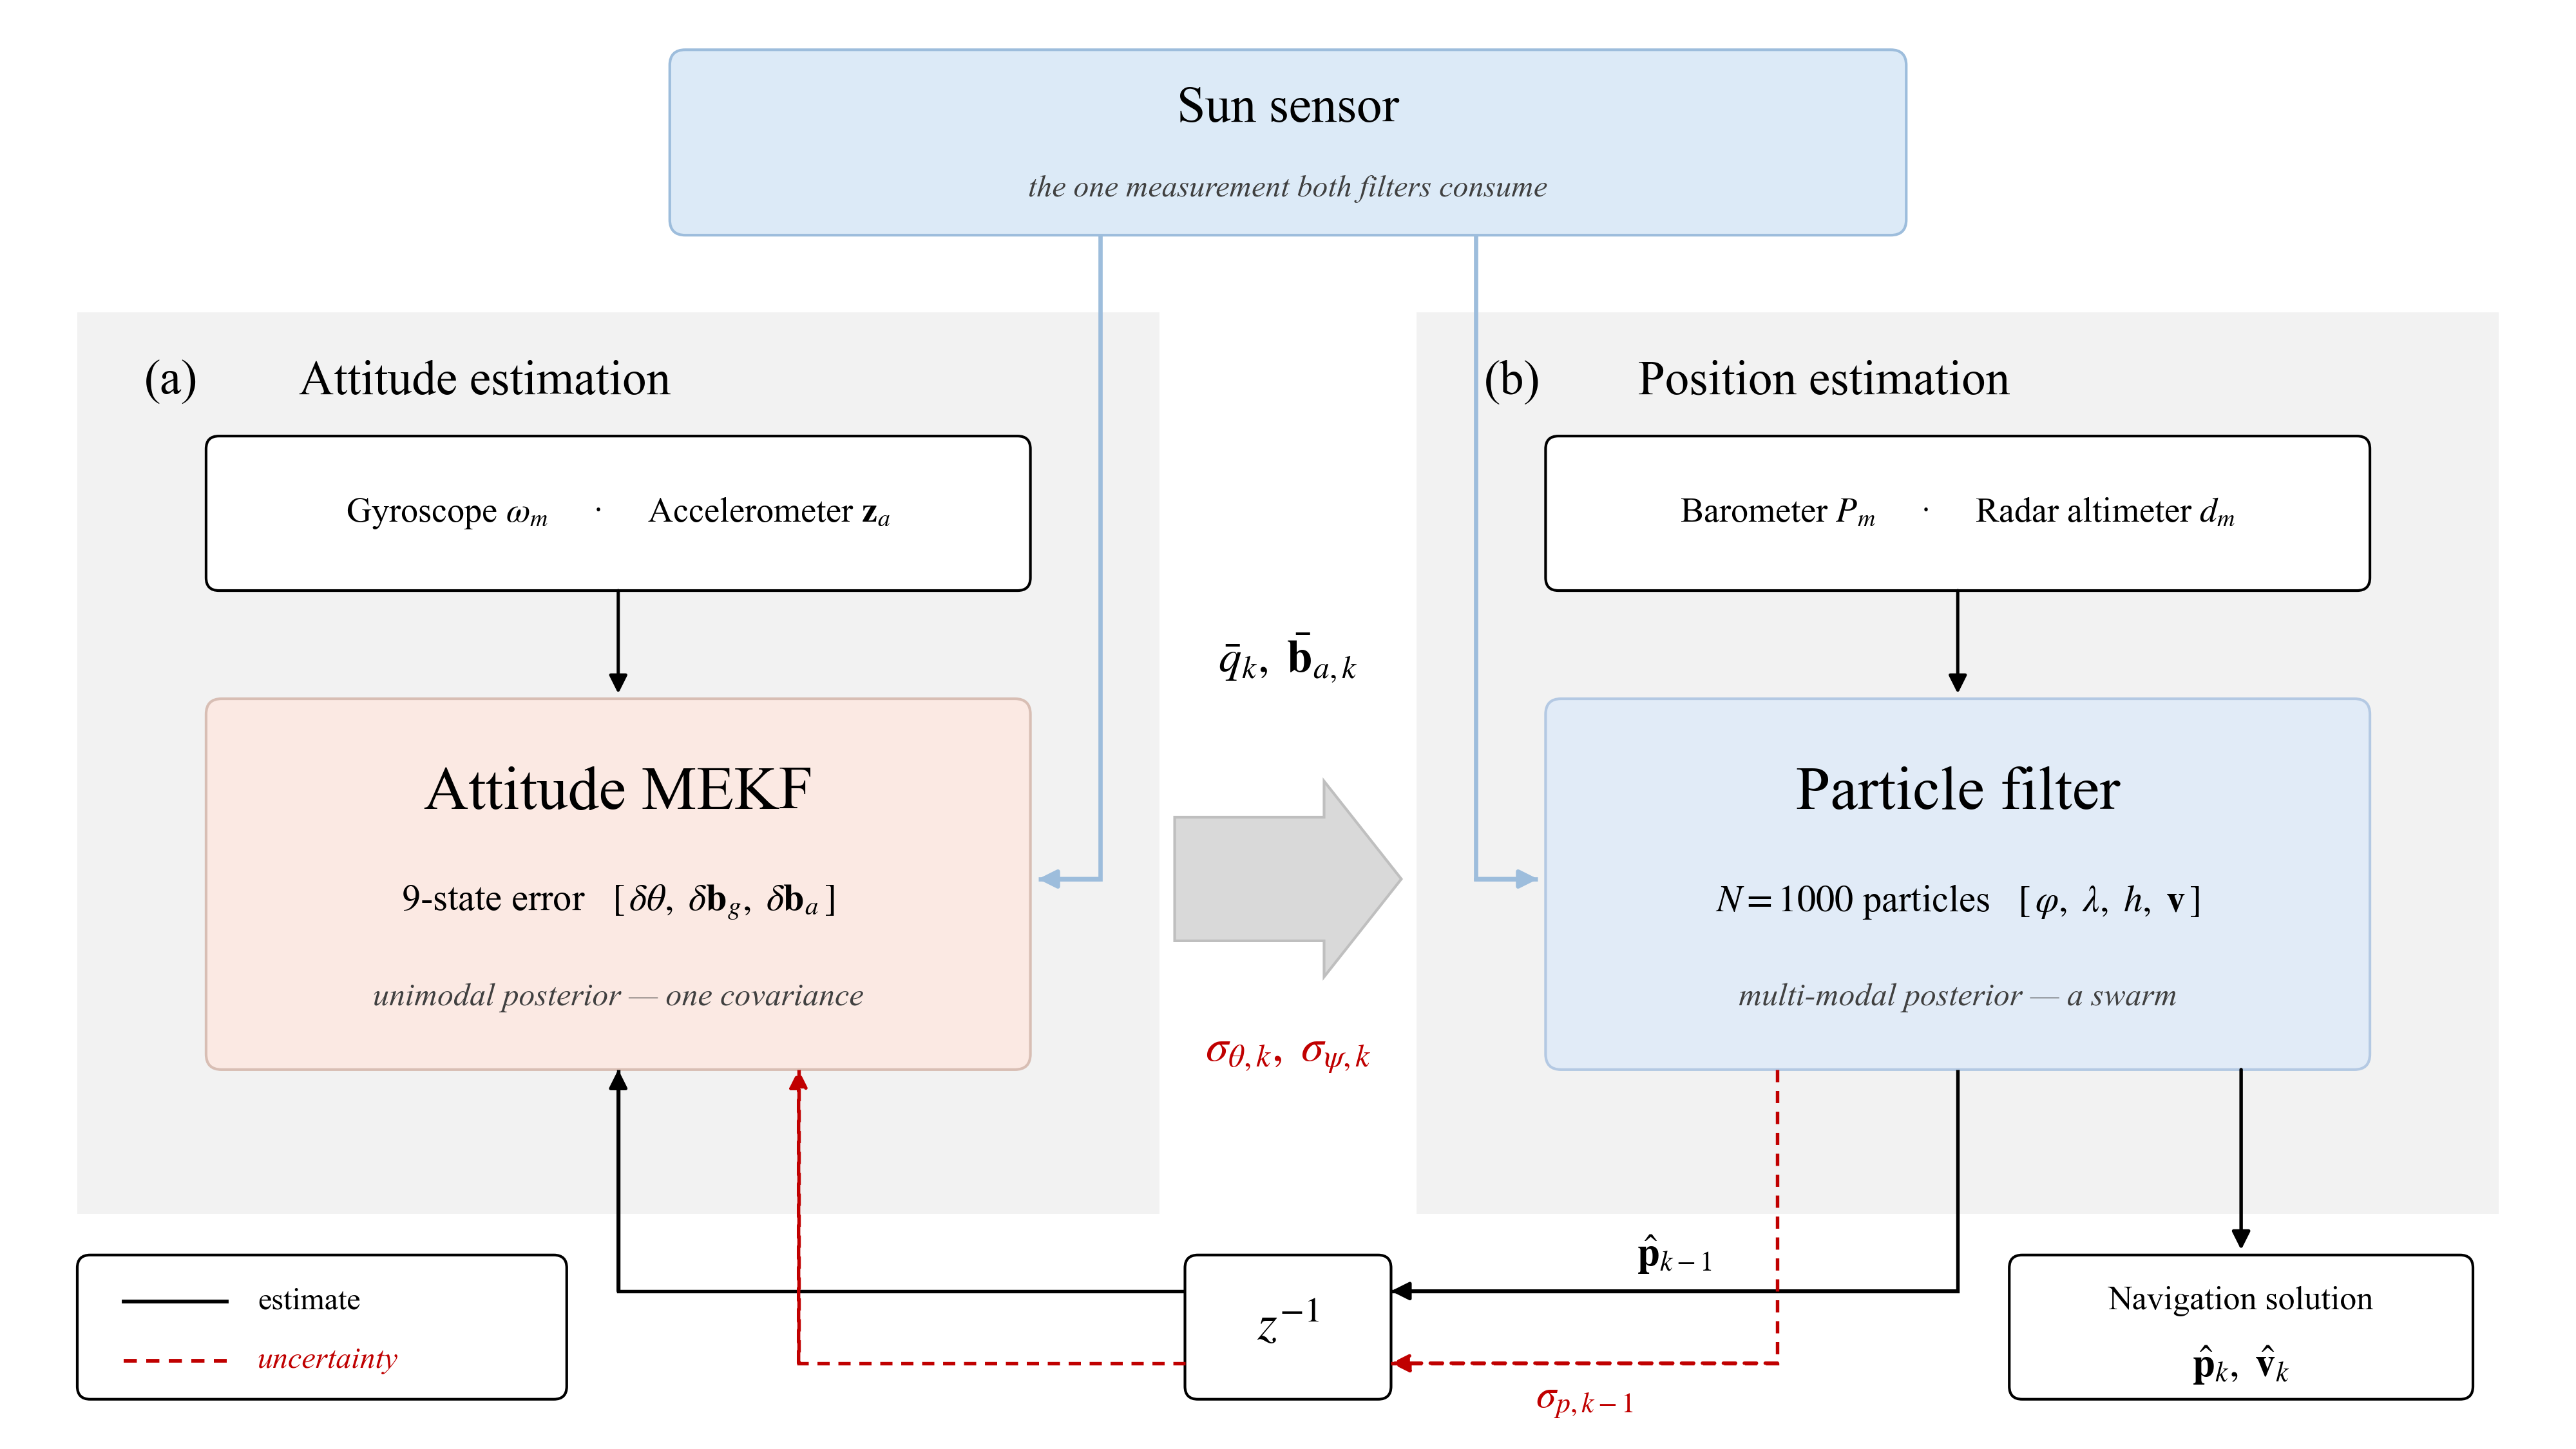
\includegraphics[width=1.0\linewidth,height=0.28\textheight,keepaspectratio]{architecture.png}
\caption{Estimation architecture: the attitude MEKF (a), carrying a nine-state error and a
single covariance, and the position particle filter (b), carrying 1000 particles over
position and velocity. Solid arrows are estimates, dashed red arrows are
uncertainties.\label{fig:architecture}}
\end{figure}

Within each epoch $k$:
\begin{enumerate}
\item the local vertical and the Sun direction are evaluated at the position estimate
produced by the particle filter at epoch $k-1$;
\item the MEKF runs its predict, correct and reset cycle on the gyroscope, the
accelerometer and the Sun sensor;
\item the quaternion, the accelerometer bias and the attitude uncertainty are handed to the
particle filter;
\item the particle filter propagates the swarm and re-weights it against the barometer, the
altimeter and the Sun angles;
\item the resulting position estimate and its spread are stored as the references of step 1
at the next epoch.
\end{enumerate}

\subsection{Attitude Estimation: the Multiplicative Extended Kalman Filter}

The MEKF~\cite{Lefferts1982} is the state-of-the-art variant of the Kalman filter for
quaternion-based attitude estimation.
It propagates with the exact nonlinear kinematics a nominal state
$\bar{\mathbf{X}}=[\bar{\mathbf{q}}^\top,\bar{\mathbf{b}}_g^\top,\bar{\mathbf{b}}_a^\top]^\top$,
the quaternion and the gyroscope and accelerometer biases, and estimates the Gaussian
error state $\delta\mathbf{X}=[\delta\boldsymbol{\theta}^\top,\delta\mathbf{b}_g^\top,
\delta\mathbf{b}_a^\top]^\top$ $\in\mathbb{R}^9$, with covariance $\mathbf{P}$, where
$\mathbf{q}^{true}=\bar{\mathbf{q}}\otimes\mathbf{q}\{\delta\boldsymbol{\theta}\}$ and
$\mathbf{q}\{\cdot\}$ maps a rotation vector to a unit quaternion~\cite{Markley2003}.

\paragraph{Prediction}
With the bias-corrected gyroscope rate $\boldsymbol{\omega}_k=\boldsymbol{\omega}_{m,k}
-\bar{\mathbf{b}}_g$, the nominal quaternion is advanced as
$\bar{\mathbf{q}}_k=\bar{\mathbf{q}}_{k-1}\otimes\mathbf{q}\{\boldsymbol{\omega}_k\Delta t\}$
and the nominal biases are held constant.
The error state evolves as $\dot{\delta\boldsymbol{\theta}}=-[\boldsymbol{\omega}\times]
\delta\boldsymbol{\theta}-\delta\mathbf{b}_g-\mathbf{n}_g$, with the biases as random walks,
so that
\begin{equation}
\mathbf{P}_k^-=\mathbf{F}\mathbf{P}_{k-1}\mathbf{F}^\top+\mathbf{Q},\qquad
\mathbf{F}=\begin{bmatrix}\mathbf{I}_3-\Delta t[\boldsymbol{\omega}\times] &
-\Delta t\,\mathbf{I}_3 & \mathbf{0}_3\\
\mathbf{0}_3 & \mathbf{I}_3 & \mathbf{0}_3\\
\mathbf{0}_3 & \mathbf{0}_3 & \mathbf{I}_3\end{bmatrix}.
\end{equation}
The process-noise covariance is obtained with the Van Loan construction~\cite{VanLoan1978},
integrating the noise together with the dynamics over the step.
Since the dynamics matrix of the attitude and gyro-bias pair is nilpotent, its transition
matrix is exactly $\boldsymbol{\Phi}(\tau)=\mathbf{I}_6+\mathbf{A}\tau$, and integrating
$\boldsymbol{\Phi}\,\mathrm{blkdiag}(\sigma_g^2\mathbf{I}_3,\sigma_{bg}^2\mathbf{I}_3)\,
\boldsymbol{\Phi}^\top$ over $[0,\Delta t]$ gives
\begin{equation}
\mathbf{Q}=\begin{bmatrix}
(\sigma_g^2\Delta t+\frac13\sigma_{bg}^2\Delta t^3)\,\mathbf{I}_3 &
-\frac12\sigma_{bg}^2\Delta t^2\,\mathbf{I}_3 & \mathbf{0}_3\\
-\frac12\sigma_{bg}^2\Delta t^2\,\mathbf{I}_3 & \sigma_{bg}^2\Delta t\,\mathbf{I}_3 &
\mathbf{0}_3\\
\mathbf{0}_3 & \mathbf{0}_3 & \sigma_{ba}^2\Delta t\,\mathbf{I}_3
\end{bmatrix},
\end{equation}
with $\sigma_g$ the gyroscope white noise and $\sigma_{bg}$, $\sigma_{ba}$ the bias
random-walk intensities of Table~\ref{tab:sensors}.

\paragraph{Measurement models}
The accelerometer measures gravity along the local up-versor $\hat{\mathbf{u}}(\mathbf{p})$, and
the Sun sensor the Sun direction $\hat{\mathbf{s}}_{VCVF}(\mathbf{p})$, both resolved in body
axes, $\hat{\mathbf{s}}_B=\mathbf{R}(\bar{\mathbf{q}})^\top\hat{\mathbf{s}}_{VCVF}(\mathbf{p})$:
\begin{gather}
\hat{\mathbf{z}}_a=\hat{\mathbf{g}}_B+\bar{\mathbf{b}}_a,\quad
\hat{\mathbf{g}}_B=g_0\mathbf{R}(\bar{\mathbf{q}})^\top\hat{\mathbf{u}}(\mathbf{p}),\qquad
\mathbf{H}_a=\begin{bmatrix}[\hat{\mathbf{g}}_B\times] & \mathbf{0}_3 & \mathbf{I}_3
\end{bmatrix},\\
\hat{\mathbf{z}}_s=\begin{bmatrix}\operatorname{atan2}(\hat s_{B,y},\hat s_{B,x})\\
\arcsin\hat s_{B,z}\end{bmatrix},\qquad
\mathbf{H}_s=\begin{bmatrix}\mathbf{J}_{ae}[\hat{\mathbf{s}}_B\times] &
\mathbf{0}_{2\times3} & \mathbf{0}_{2\times3}\end{bmatrix},
\end{gather}
with $\mathbf{J}_{ae}=\partial(az,el)/\partial\hat{\mathbf{s}}_B$, whose azimuth row scales as
$1/\cos(el)$, and noise covariances $\mathbf{R}_a=\mathrm{diag}(\sigma_w^2+\sigma_{k,i}^2)$,
where $\sigma_{k,i}$ accounts for the kinematic acceleration of the swinging vehicle, and
$\mathbf{R}_s=\sigma_s^2\mathbf{I}_2$.
Each correction computes $\mathbf{K}=\mathbf{P}\mathbf{H}^\top(\mathbf{H}\mathbf{P}
\mathbf{H}^\top+\mathbf{R})^{-1}$ and $\delta\hat{\mathbf{X}}=\mathbf{K}(\mathbf{z}-
\hat{\mathbf{z}})$, folds the error into the nominal state,
$\bar{\mathbf{q}}\leftarrow\bar{\mathbf{q}}\otimes\mathbf{q}\{\delta\hat{\boldsymbol{\theta}}\}$
and $\bar{\mathbf{b}}_\bullet\leftarrow\bar{\mathbf{b}}_\bullet+\delta\hat{\mathbf{b}}_\bullet$,
updates $\mathbf{P}$ in Joseph form, and resets the error state to zero.

\subsection{Position Estimation: the Particle Filter}

The terrain-relative likelihood is multi-modal in horizontal position, which no single
Gaussian can represent.
The particle filter~\cite{Gordon1993,Arulampalam2002} represents the posterior by $N=1000$
weighted samples, each a hypothesis on the translational state
$\mathbf{X}^i=\{\mathbf{p}^i,\mathbf{v}^i\}$, $\mathbf{p}^i=[\varphi^i,\lambda^i,h^i]$.
In this way, several possible positions of the balloon can be kept at the same time, until
the measurements make one of them clearly more likely than the others
(Fig.~\ref{fig:multimodality}).

\Fig{multimodality.png}{0.96}{Multimodal posterior represented by the particle swarm: competing
location hypotheses coexist as clusters until the measurements single one
out.\label{fig:multimodality}}

\paragraph{Propagation}
Each particle is propagated through the translational dynamics of Eq.~\eqref{eq:dynamics},
pushed by the wind, with the atmosphere $(P^i,\rho^i,T^i,\mathbf{W}^i)$ read at its own
position from the nominal, mean fields of the Venus Climate Database~\cite{Lebonnois2023}.
Volume, reference area, mass and forces are evaluated per particle, and
\begin{equation}
\mathbf{a}^i=\frac{\mathbf{F}_{grav}^i+\mathbf{F}_{buoy}^i+\mathbf{F}_{drag}^i}{m_{tot}^i}
-\boldsymbol{\omega}_p\times(\boldsymbol{\omega}_p\times\mathbf{r}^i)
-2\,\boldsymbol{\omega}_p\times\mathbf{v}^i+\boldsymbol{\eta}_a^i
\end{equation}
is integrated with an Euler step, the process noise $\boldsymbol{\eta}_a^i$ keeping the swarm
from collapsing onto a single trajectory.
Every particle thus flies the nominal atmosphere while the truth flies the perturbed one, and
this discrepancy is the dominant model error of the estimator.

\paragraph{Measurement update}
The barometer innovation is a direct map comparison, $\nu_{bar}^i=P_m-P_{LUT}(\mathbf{p}^i,t)$.
The altimeter innovation stretches the vertical terrain clearance $\hat h_\perp^i$ of the map
by the tilt of the body $-Z$ axis $\mathbf{n}=-\mathbf{R}(\bar{\mathbf{q}})\hat{\mathbf{z}}$,
\begin{equation}
\nu_{alt}^i=d_m-\frac{\hat h_\perp^i}{\cos\gamma^i},\qquad
\cos\gamma^i=-\left[\mathbf{R}_{VCVF\to ENU}(\mathbf{p}^i)\,\mathbf{n}\right]_U.
\end{equation}
The Sun sensor is informative for position only in the local horizon frame.
The measured Sun direction and the specific force, de-biased with the MEKF estimate, are
rotated into VCVF with the shared attitude,
\begin{equation}
\hat{\mathbf{u}}_{meas}=\mathbf{R}(\bar{\mathbf{q}})\frac{\mathbf{z}_a-\bar{\mathbf{b}}_a}
{\|\mathbf{z}_a-\bar{\mathbf{b}}_a\|},\qquad
\hat{\mathbf{s}}_{meas}=\mathbf{R}(\bar{\mathbf{q}})
\begin{bmatrix}\cos el\cos az\\ \cos el\sin az\\ \sin el\end{bmatrix},
\end{equation}
and the measured azimuth and elevation are taken in the ENU triad built on
$\hat{\mathbf{u}}_{meas}$; the predicted angles of each particle follow from the ephemeris Sun
position in that particle's own ENU frame, so that the innovations $\nu_{az}^i$,
$\nu_{el}^i$ depend on its absolute latitude and longitude.

\paragraph{Weighting and resampling}
The active channels are combined into
$D^i=\boldsymbol{\nu}^{i\top}\mathbf{R}^{-1}\boldsymbol{\nu}^i$, with
$\mathbf{R}=\mathrm{diag}(\sigma_{bar}^2,\sigma_{alt}^2,\sigma_{az}^2,\sigma_{el}^2)$, and
weighted by a heavy-tailed, tempered Student's-$t$ likelihood,
\begin{equation}
\log w_k^i=\log w_{k-1}^i-\beta\,\frac{\nu_t+m}{2}\log\left(1+\frac{D^i}{\nu_t}\right),
\end{equation}
with $\nu_t$ the degrees of freedom, $\beta$ the tempering exponent and $m$ the number of
active channels.
The heavy tail keeps an occasional anomalous match from killing a particle.
The tempering $\beta<1$ makes each update only a small correction of the weights, so that
a particle is judged on the accumulated evidence of many successive epochs rather than on a
single one: the weights then reflect how well the particle matches the terrain profile
travelled over a long stretch of trajectory, which carries much more topographic
information than a point-by-point comparison.
Since the residuals are correlated over hundreds of seconds while the update runs at
\SI{10}{Hz}, an untempered likelihood would also treat correlated samples as independent and
collapse the swarm within seconds.
Degeneracy is measured by the effective sample size~\cite{Kong1994,Arulampalam2002},
\begin{equation}
N_{eff}=\frac{1}{\sum_{i=1}^N(w_k^i)^2},
\end{equation}
which equals $N$ for uniform weights and 1 when a single particle carries them all.
When $N_{eff}<0.5N$ the swarm is regenerated by systematic resampling~\cite{Kitagawa1996},
the weights are reset to $1/N$, and each position is roughened~\cite{Gordon1993} by a
Gaussian displacement of \SI{0.05}{\degree} to counteract sample impoverishment.
The estimate is a weighted mean over the particles within \SI{25}{km} of the most probable
one, while its covariance $\boldsymbol{\Sigma}_p$ is computed over the whole swarm.

\paragraph{Remark on the longitude problem and the role of the Sun sensor}
With the barometer and the altimeter alone, the estimate can drift over flat terrain and
become trapped in a local minimum of the topography (Fig.~\ref{fig:trapping}): four runs out
of ten diverge in this way, through a longitude lock that is never corrected.
The Sun channels, which have no local minima and depend on absolute longitude, are the only
measurement able to detect and correct such a divergence.

\Fig{terrain_trapping.png}{1.00}{Terrain trapping with altimeter and barometer only: the
estimate stays locked on one side of a massif (4 runs out of 10 diverge), motivating the Sun
channel.\label{fig:trapping}}

\subsection{Uncertainty Exchange Between the Two Filters}

In the cascade, point estimates and their uncertainties cross the interface
(Table~\ref{tab:exchange}).
The uncertainty of each transferred quantity is added to the receiving filter's
measurement noise, recomputed at every epoch.

\begin{table}[H]\centering\small
\caption{Quantities exchanged between the two estimators at each epoch. Three of the five
entries are uncertainties rather than values.}\label{tab:exchange}
\begin{tabular}{@{}llp{8.5cm}@{}}
\toprule Quantity & Direction & Purpose in the receiving filter\\\midrule
$\bar q_k$ & MEKF $\to$ PF & tilts the altimeter slant range; builds the measured horizon frame\\
$\bar b_{a,k}$ & MEKF $\to$ PF & de-biases the specific force before the vertical is reconstructed\\
$\sigma_{\theta,k}$ & MEKF $\to$ PF & inflates the Sun-channel noise\\
$\hat p_k$ & PF $\to$ MEKF & builds the local-vertical and Sun references\\
$\sigma_{p,k}$ & PF $\to$ MEKF & inflates the accelerometer and Sun measurement noise\\\bottomrule
\end{tabular}
\end{table}

\paragraph{Attitude uncertainty into the particle filter}
For particle $i$, the attitude covariance $\mathbf{P}_{\theta\theta}$ is projected on its own
local vertical $\hat{\mathbf{u}}_B^{(i)}=\mathbf{R}(\bar{\mathbf{q}})^\top
\hat{\mathbf{u}}(\mathbf{p}^i)$ to give the yaw uncertainty, the rest of the trace being
attributed to the two tilt axes together with the accelerometer noise.
Since a tilt moves the elevation one-for-one and the azimuth by $1/\cos(el)$, while a yaw
moves only the azimuth, the Sun channels use
\begin{gather}
\sigma_{el}=\sqrt{\sigma_s^2+v_{tilt}},\qquad
\sigma_{az}=\sqrt{\sigma_s^2+\sigma_\psi^2+\frac{v_{tilt}}{\cos^2el}},\\
\sigma_\psi^2=\hat{\mathbf{u}}_B^{(i)\top}\mathbf{P}_{\theta\theta}\hat{\mathbf{u}}_B^{(i)},\quad
v_{tilt}=\frac{\mathrm{tr}\,\mathbf{P}_{\theta\theta}-\sigma_\psi^2}{2}
+\frac{\sigma_w^2}{g_0^2}.
\end{gather}

\paragraph{Position uncertainty into the MEKF}
The swarm covariance is converted into the horizontal arc length
$\sigma_p^2=(r\sigma_\varphi)^2+(r\cos\varphi\,\sigma_\lambda)^2$, with
$r=R_V+h\approx\SI{6107}{km}$.
For the Sun sensor it produces a parallax $\sigma_{par}=(180/\pi)\,\sigma_p/d_\odot$ degrees,
with $d_\odot\approx\SI{1.08e8}{km}$; for the accelerometer it tilts the local vertical by
$\sigma_u=\sigma_p/(\sqrt2\,r)$ per horizontal axis.
The two covariances become
\begin{align}
\mathbf{R}_s&=\mathrm{diag}\left(\sigma_s^2+\frac{\sigma_{par}^2}{\cos^2el},\
\sigma_s^2+\sigma_{par}^2\right),\\
\mathbf{R}_a&=\mathrm{diag}(\sigma_w^2+\sigma_{k,i}^2)+(g_0\sigma_u)^2
\left(\mathbf{I}_3-\hat{\mathbf{g}}\hat{\mathbf{g}}^\top\right),
\end{align}
the tilt term being injected in rank-two form so that the radial channel, which carries the
accelerometer-bias information, is untouched.
The local vertical is $r/d_\odot\approx1.8\times10^4$ times more sensitive to a position error
than the Sun direction, and the position error is correlated in time: the MEKF therefore
corrects with the Sun sensor every \SI{10}{s} and with the accelerometer only every
\SI{1000}{s}.

\section{Simulations and Results}\label{sec:results}
\subsection{Simulation Setup}

After a reference run (Section~\ref{sec:refrun}), the estimator is therefore assessed through
Monte Carlo campaigns, organised as a sensitivity analysis on the two main assumptions: the knowledge of the atmosphere (Section~\ref{sec:sens_atm}) and the
accuracy of the Sun sensor (Section~\ref{sec:sens_sun}).

Each configuration is simulated over one hundred independent runs.
Each run starts at the epoch of Table~\ref{tab:scenario}, with the balloon at \SI{58}{km} of
altitude and \SI{0}{\degree} of longitude, a latitude drawn uniformly between
\SI{-20}{\degree} and \SI{20}{\degree}, and its own atmospheric-perturbation and sensor-noise
seeds (Fig.~\ref{fig:campaign}).
Each run simulates \SI{100}{h} of flight at $\Delta t=\SI{0.1}{s}$, within which the
far-side window lasts about \SI{65}{h}, the Sun setting about \SI{46}{h} after the link is
lost.
The estimator is the full architecture of Section~\ref{sec:estimation}, with $N=1000$
particles and the cadences of Section~\ref{sec:estimation}.
The initial attitude of the MEKF is computed with the TRIAD method~\cite{Black1964} from
the first Sun-sensor and accelerometer readings.
The MEKF is started \SI{2}{h} before the blackout, while the position is still known, so that
its initial transient has settled when the particle filter takes over; the particles are
initialised about the last known state with $\sigma_\varphi=\sigma_\lambda=\SI{0.1}{\degree}$,
$\sigma_h=\SI{50}{m}$ and $\sigma_v=\SI{1}{m\,s^{-1}}$.

\Fig{campaign_trajectories.png}{0.86}{Ground tracks of 10 Monte Carlo runs, launched at
longitude $0^\circ$ with latitude uniform in $[-20^\circ,20^\circ]$.\label{fig:campaign}}

Every run is scored over the sunlit arc only, on three statistics:
\begin{itemize}
\item \textbf{Lost runs}, whose position error crosses a \SI{500}{km} threshold before sunset
and does not recover, counted out of one hundred;
\item \textbf{RMSE}, the position root-mean-square error over the sunlit arc, averaged over
the runs that are not lost;
\item \textbf{$3\sigma$ coverage}, the fraction of sunlit epochs at which the true position
error lies within the filter's own $3\sigma$ bound, averaged over the runs that are not lost.
\end{itemize}

\subsection{Reference Run}\label{sec:refrun} % formerly Sec. 3.6

Before the campaigns, the coupled estimator is tested on a single reference run.
Figure~\ref{fig:ref_att} zooms into a ten-minute window late in the sunlit arc: roll and pitch
oscillate by a few tenths of a degree as the balloon swings, and the MEKF follows that
oscillation with the true value inside its declared $3\sigma$ band; yaw, driven by the much
larger and slower rotation of the heading, is reproduced with no visible lag.

\Fig{singlerun_attitude_zoom.png}{0.81}{Single run: estimated vs. true roll, pitch and yaw over
a 10 min window, with the MEKF $\pm3\sigma$ band.\label{fig:ref_att}}

The particle-filter mean follows the true latitude and longitude closely, and the altitude
estimate follows the oscillations of the balloon around its float level
(Fig.~\ref{fig:ref_pos}).
Figure~\ref{fig:ref_err} quantifies the resulting accuracy: a horizontal RMSE of
\SI{23.7}{km}, with a worst-case excursion of about \SI{80}{km}, and an error that stays
within the filter's own $3\sigma$ bound.

\Fig{singlerun_position_estimation.png}{0.81}{Single run: particle-filter position mean vs.
truth (latitude, longitude, altitude).\label{fig:ref_pos}}
\Fig{singlerun_position_error.png}{0.81}{Single run: horizontal position error (RMSE 23.7 km,
maximum about 80 km) and per-axis error against the declared $\pm3\sigma$.\label{fig:ref_err}}
\Fig{singlerun_particle_tracking.png}{1.00}{Particle swarm over the local topography at $t=57.5$
h, with true and estimated positions.\label{fig:ref_swarm}}

\subsection{Sensitivity to the Atmospheric Model}\label{sec:sens_atm}

Every result of this work already includes a persistent modelling error, since the particles
fly the mean fields of the Venus Climate Database while the truth flies its perturbed version.
This campaign degrades the onboard atmosphere further, by reading the same database five
Venus hours out of phase.
Since the database is indexed by local solar time, this corrupts the filter's knowledge of
the diurnal cycle of the atmosphere.

\Fig{atmos_sensitivity.png}{0.96}{Atmosphere campaign (100 runs): reading the database five
Venusian hours out of phase costs 7.6 km of RMSE (26.7 to 34.3 km).\label{fig:sens_atm}}

\begin{table}[H]\centering\small
\caption{Sensitivity to the fidelity of the filter's onboard atmosphere. One hundred runs per
row, sunlit arc only, identical seeds and initial latitudes.}\label{tab:sens_atm}
\begin{tabular}{@{}lccc@{}}
\toprule Atmosphere the filter propagates on & RMSE [km] & $3\sigma$ coverage [\%] & Lost\\\midrule
Nominal database & 26.7 & 88.4 & 1/100\\
Database lagged 5 Venus h & 34.3 & 75.1 & 2/100\\\bottomrule
\end{tabular}
\end{table}

The estimator is sensitive to the knowledge of the atmosphere (Table~\ref{tab:sens_atm},
Fig.~\ref{fig:sens_atm}): the lagged database worsens the RMSE by \SI{7.6}{km} and lowers
the $3\sigma$ coverage by thirteen percentage points, since the particles are propagated on
a wind that departs further from the real one.
The RMSE nonetheless remains within the \SI{50}{km} requirement.
The number of lost runs, one or two out of one hundred, against four out of ten in the
configuration without the Sun channels in the position update
(Section~\ref{sec:estimation}), reflects the importance of the double use of the Sun sensor,
in both the attitude and the position filter.
A way to reduce the gap between the modelled and the real atmosphere is proposed in
Section~\ref{sec:conclusions}.

\subsection{Sensitivity to the Sun Sensor Noise}\label{sec:sens_sun}

The Sun sensor has not been designed in detail, and the baseline
$\sigma_s=\SI{1e-4}{\degree}$ may not be achievable through the cloud deck.
This campaign repeats the protocol over three decades of $\sigma_s$ with the nominal atmosphere model.

\begin{table}[H]\centering\small
\caption{Sensitivity to the Sun-sensor noise $\sigma_s$. One hundred runs per row, sunlit arc
only, nominal atmosphere throughout.}\label{tab:sens_sun}
\begin{tabular}{@{}lccc@{}}
\toprule $\sigma_s$ & RMSE [km] & $3\sigma$ coverage [\%] & Lost\\\midrule
$1\times10^{-4}$ deg & 26.7 & 88.4 & 1/100\\
$1\times10^{-2}$ deg & 27.4 & 91.8 & 2/100\\
$1\times10^{-1}$ deg & 25.7 & 95.3 & 1/100\\\bottomrule
\end{tabular}
\end{table}


\Fig{sun_sensitivity.png}{0.96}{Sun-sensor campaign (100 runs per row): across three decades of
noise the RMSE moves by only 1.7 km.\label{fig:sens_sun}}

Across three decades of sensor noise the results do not change (Table~\ref{tab:sens_sun},
Fig.~\ref{fig:sens_sun}): the RMSE stays between \SI{25.7}{km} and \SI{27.4}{km}, a spread
of \SI{1.7}{km} that is not even monotonic in $\sigma_s$, and the number of lost runs stays
at one or two out of a hundred.
The estimate is always carried mainly by the altimeter and
the barometer, which constrain the position at a much finer horizontal scale than the Sun
direction: a difference of a fraction of a degree in Sun azimuth or elevation corresponds to
hundreds of kilometres between two particles.
The Sun channels are used only to detect and correct a divergence, when the estimate is
locked in a local topographic minimum.
For this reason the RMSE stays at the level set by the terrain-relative channels, of a few
tens of kilometres, and does not deteriorate with a worse Sun sensor.

The $3\sigma$ coverage, instead, increases with $\sigma_s$.
This is not a real improvement in the consistency of the filter: a larger sensor noise
makes the measurement covariance $\mathbf{R}$ of the particle filter larger, so the weights
discriminate less between particles and the swarm stays more dispersed, which inflates the
covariance it reports.

\section{Conclusions and Future Work}\label{sec:conclusions}

This work estimated the trajectory of a Venus aerobot across the sunlit arc of the far-side
DSN occultation with an MEKF and a particle filter coupled in cascade, validated on a
simulated truth that flies a different atmosphere from the estimator.

\subsection{Main Findings}

\begin{enumerate}
\item \textbf{The Sun channel prevents divergence.}
With the barometer and the altimeter alone four runs in ten lock onto a false terrain match
in longitude; adding the Sun channels, resolved in the local horizon frame, raises the
convergence rate from about 60\% to 98--99\% in every campaign.
\item \textbf{The estimator meets the requirement.}
The position RMSE over the sunlit arc is \SI{26.7}{km}, never worse than \SI{34.3}{km}, within
the \SI{50}{km} requirement: about a quarter of one per cent of the \SI{10000}{km} flown,
and half the \SI{47.95}{km} of Cottrill and Gu~\cite{Cottrill2024} over a horizon more than
forty times longer.
\item \textbf{Uncertainty must cross the interface.}
A cascade that hands over bare estimates makes the receiving filter overconfident;
re-injecting the transferred covariance into the measurement noise at every epoch avoids it.
\item \textbf{The accuracy is set by the atmosphere, not by the Sun sensor.}
A lagged onboard atmosphere costs \SI{7.6}{km} of RMSE, whereas three decades of Sun-sensor
noise move it by \SI{1.7}{km}: the \SI{1e-4}{\degree} baseline is not a requirement.
\end{enumerate}

\subsection{Limitations and Future Work}

\paragraph{The eclipse}
In the last \SI{19}{h} only the barometer and the altimeter remain: longitude becomes
unobservable and a false terrain lock is never corrected, so divergences rise sharply.
A smoother that also exploits the DSN fix at the end of the blackout, or a second absolute
reference available after sunset, would address it.

\paragraph{The velocity and the wind model}
No sensor measures velocity, and each particle moves with the nominal wind, so a wind error
appears as a position bias.
A slowly varying wind-bias state in each particle, informed by the position innovations,
would let the swarm learn the offset between the modelled and the real wind, reducing the
dependence on the onboard atmosphere found in Section~\ref{sec:sens_atm}.

Finally, the estimator should be tested in a higher-fidelity environment and against data
from flight-representative aerobot tests~\cite{Hall2021,Izraelevitz2025}.

{\footnotesize
\bibliographystyle{elsarticle-num}
\bibliography{references}
}

\end{document}
